%!TEX root =  ../main.tex

\chapterimage{\chapdir/pics/Northern_lights_in_Greenland} 
\mychapter{Triangles}{triangles}

Amazingly, the trigonometric functions defined by right-triangles are
meaningful on non-right triangles.  The Pythagorean theorem is actually
just a special case of the Law of Cosines.  Triangles, it seems, are the
building blocks of the universe.

Why are triangles so productive?  What is so special about triangles?
Is there another shape with such descriptive power?

\newpage
\chapterminitoc


%									11 - 1
\newpage
\section{Area Formulae}
\noindent\makebox[\textwidth]{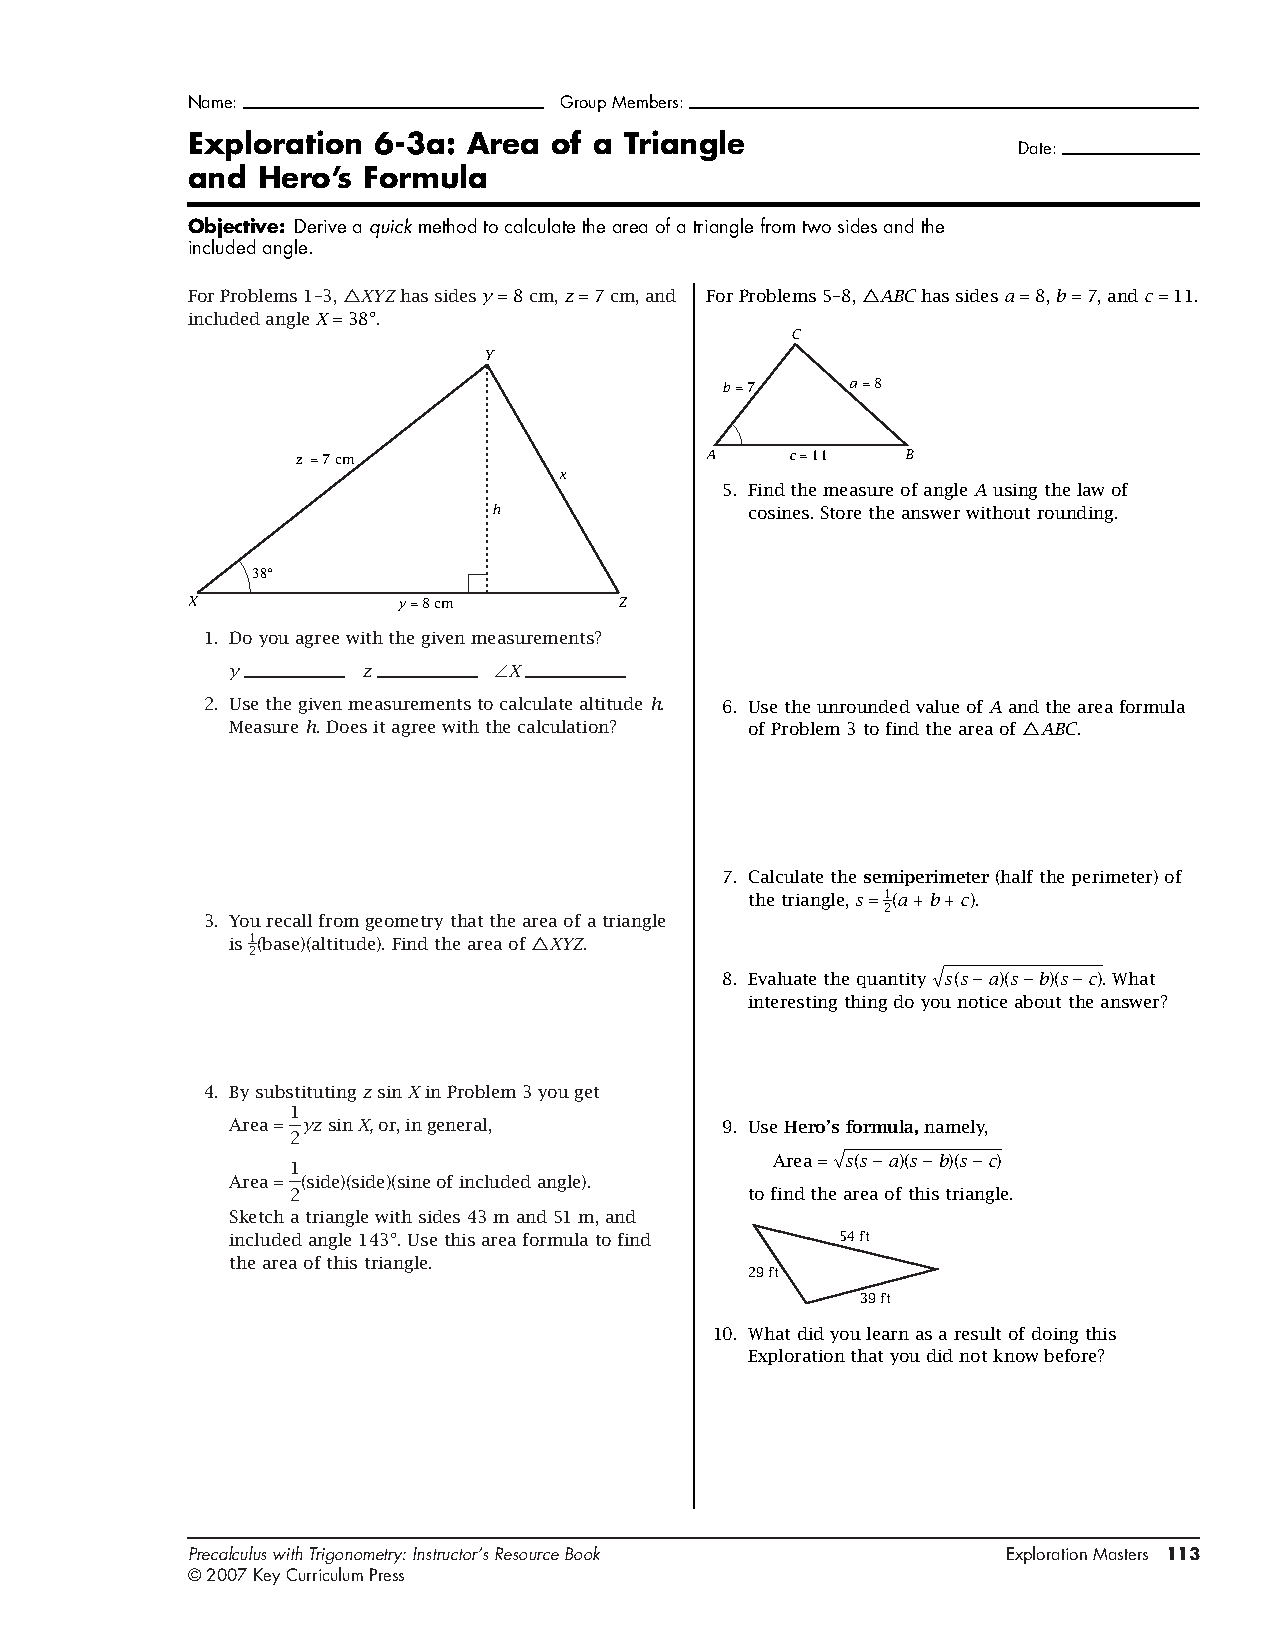
\includegraphics[width=\paperwidth]{ch11/1101p.pdf}}
\subsection{Sine Formulae}
\subsection{Heron's Formula}
\newpage
\subsection{Exercises}
To be done in Kuta


%									11 - 2
%\newpage
\invisiblesection{Law of Cosines}
\subsection{Problems}
\noindent\makebox[\textwidth]{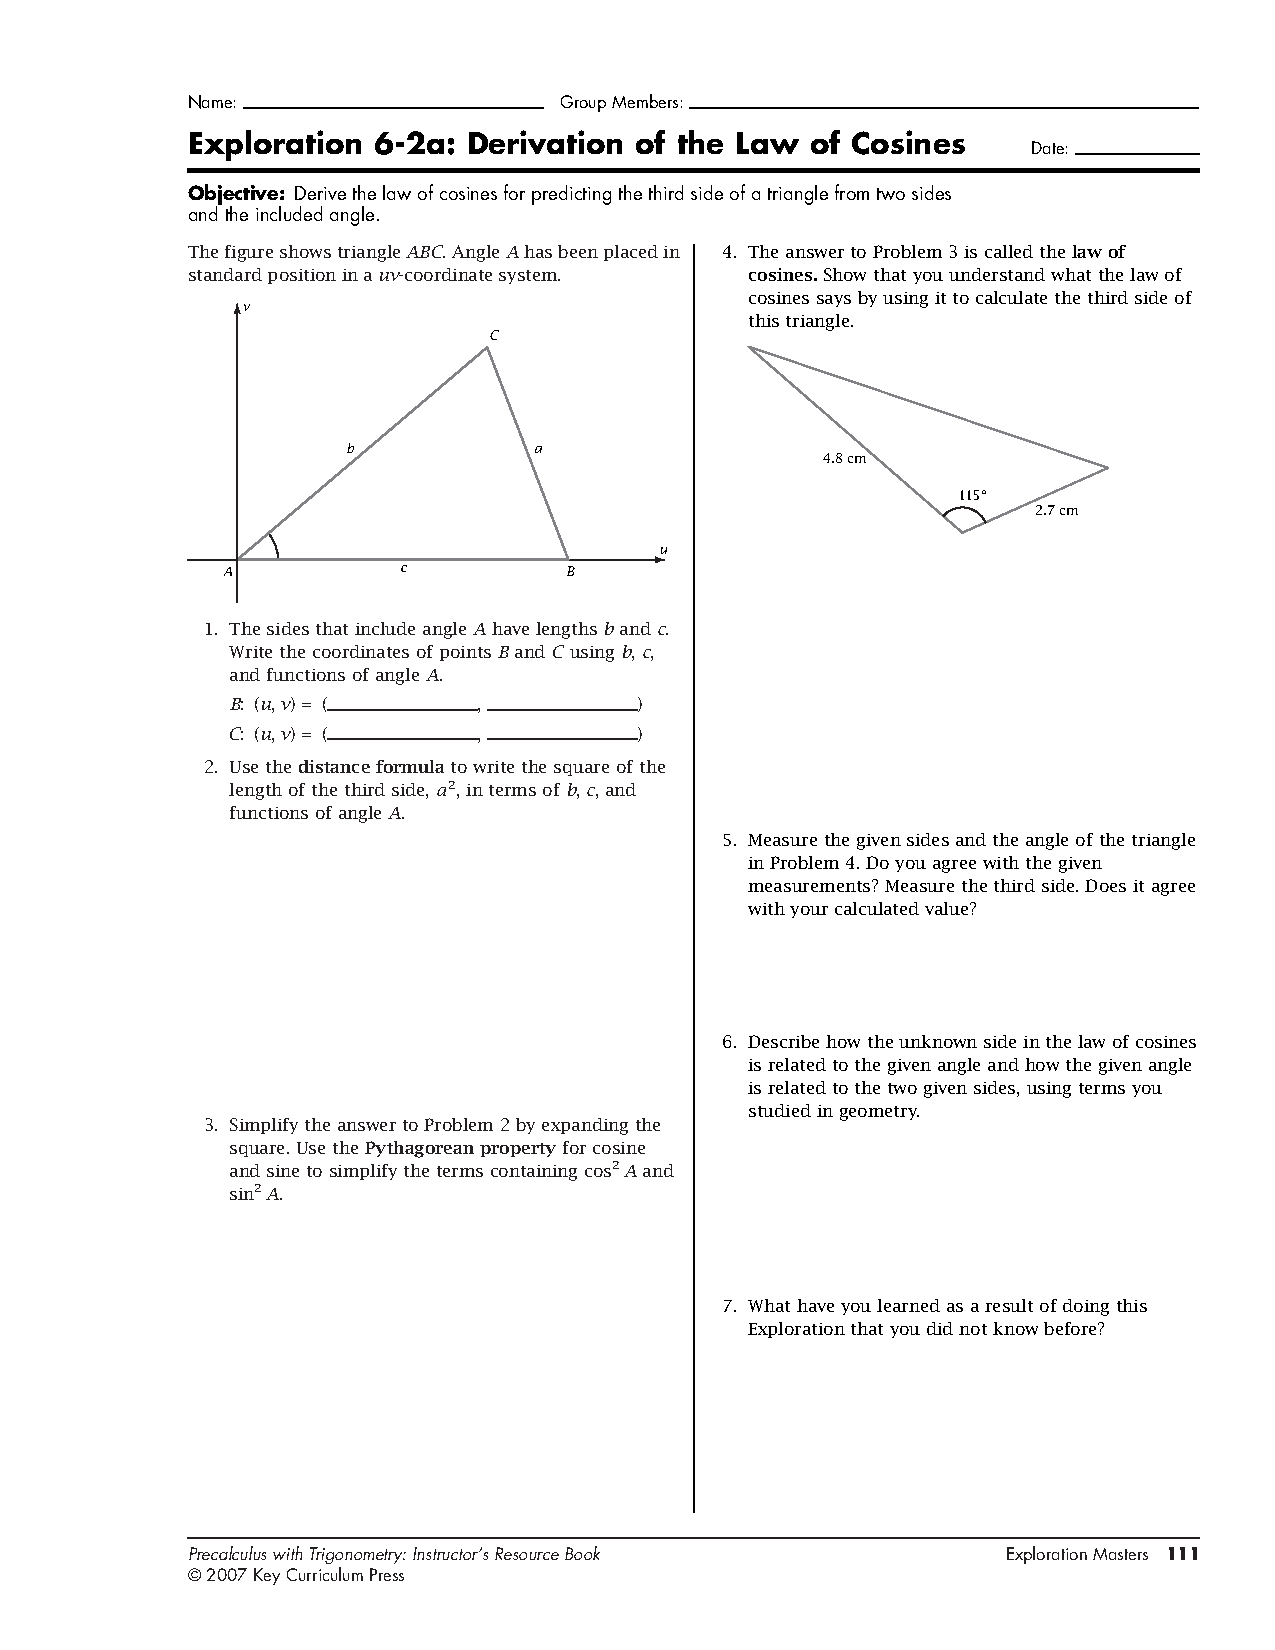
\includegraphics[width=\paperwidth]{ch11/1102p.pdf}}
\newpage
\subsection{SSS}
\subsection{SAS}
\newpage
\subsection{Exercises}
to be done in kuta

%									11 - 3
\newpage
\invisiblesection{Law of Sines}
\subsection{Problems}
\noindent\makebox[\textwidth]{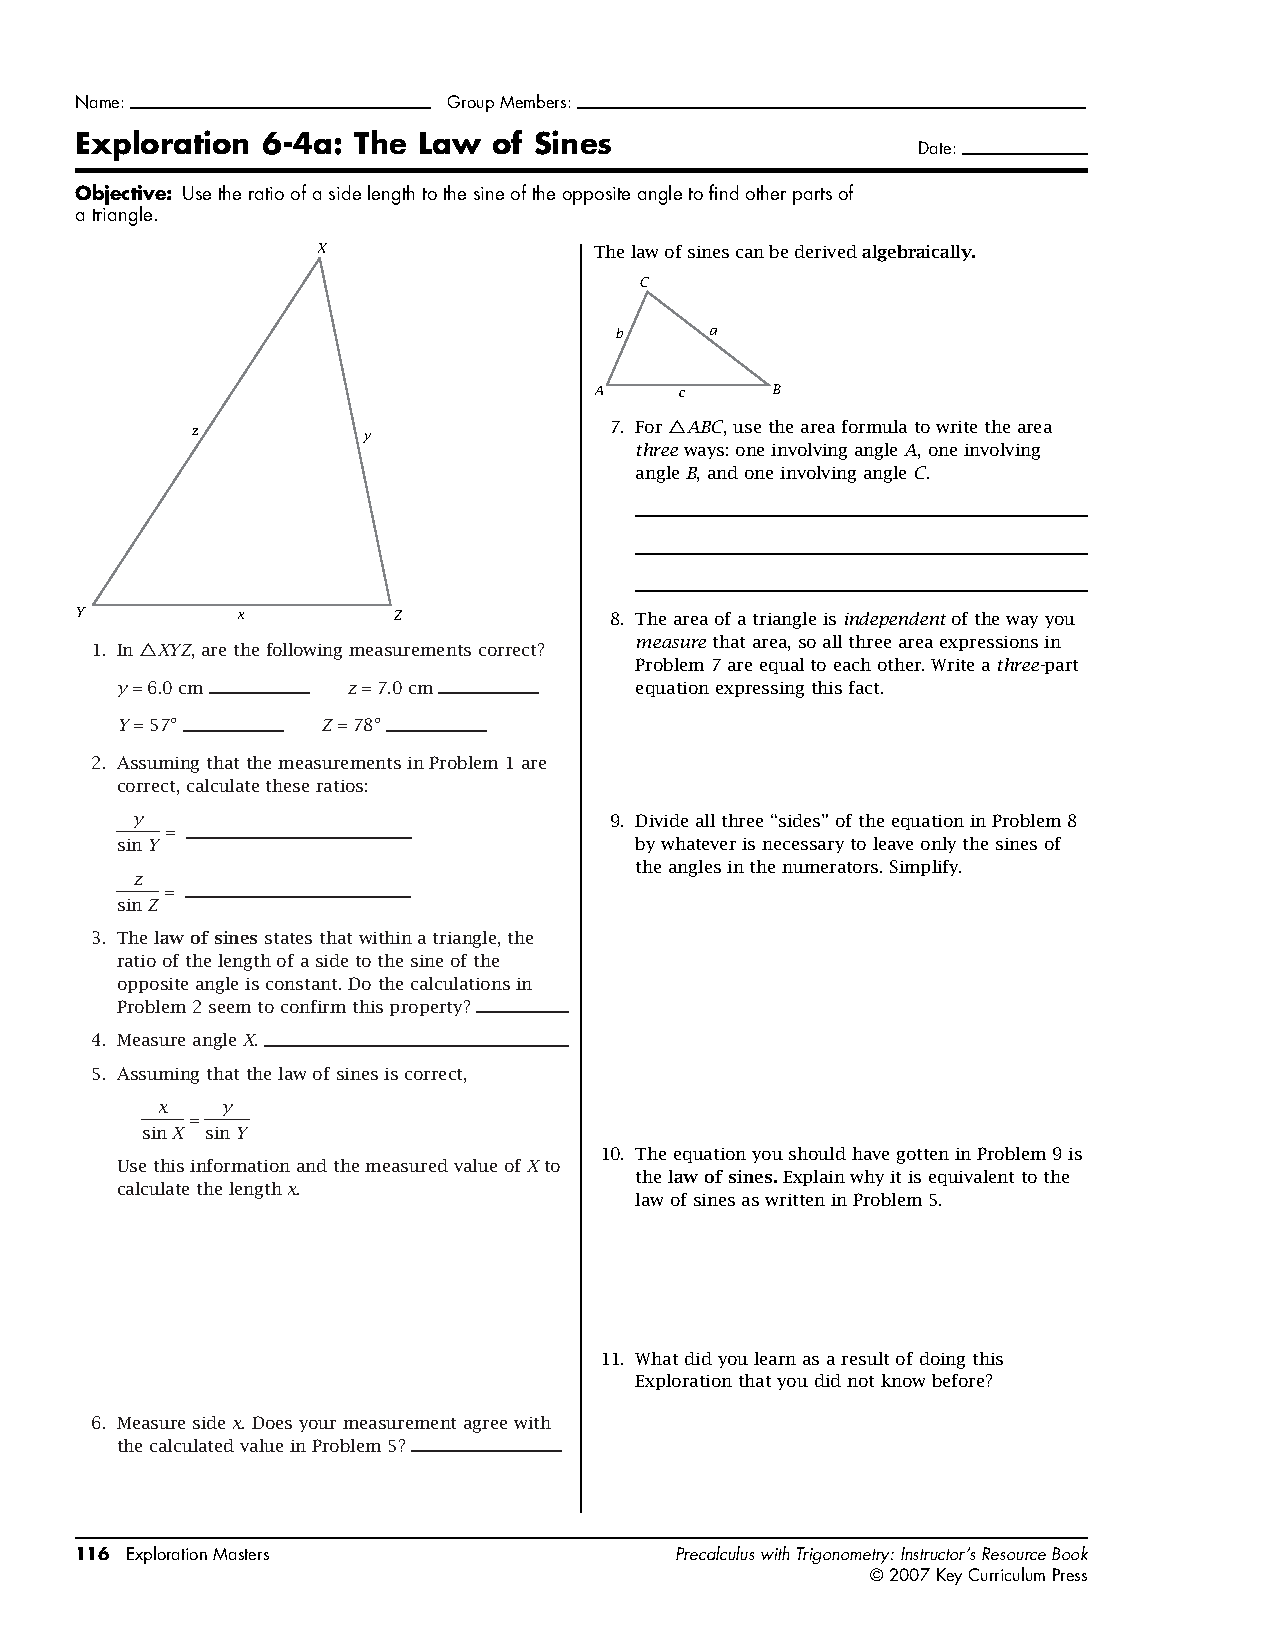
\includegraphics[width=\paperwidth]{ch11/1103p.pdf}}
\newpage
\subsection{Imagining the Height}
\subsection{SAA}
\subsection{ASA}
\newpage
\subsection{Exercises}
to be done in kuta

%									11 - 4
\newpage
\invisiblesection{The Ambiguous Case}
\subsection{Problems}
\noindent\makebox[\textwidth]{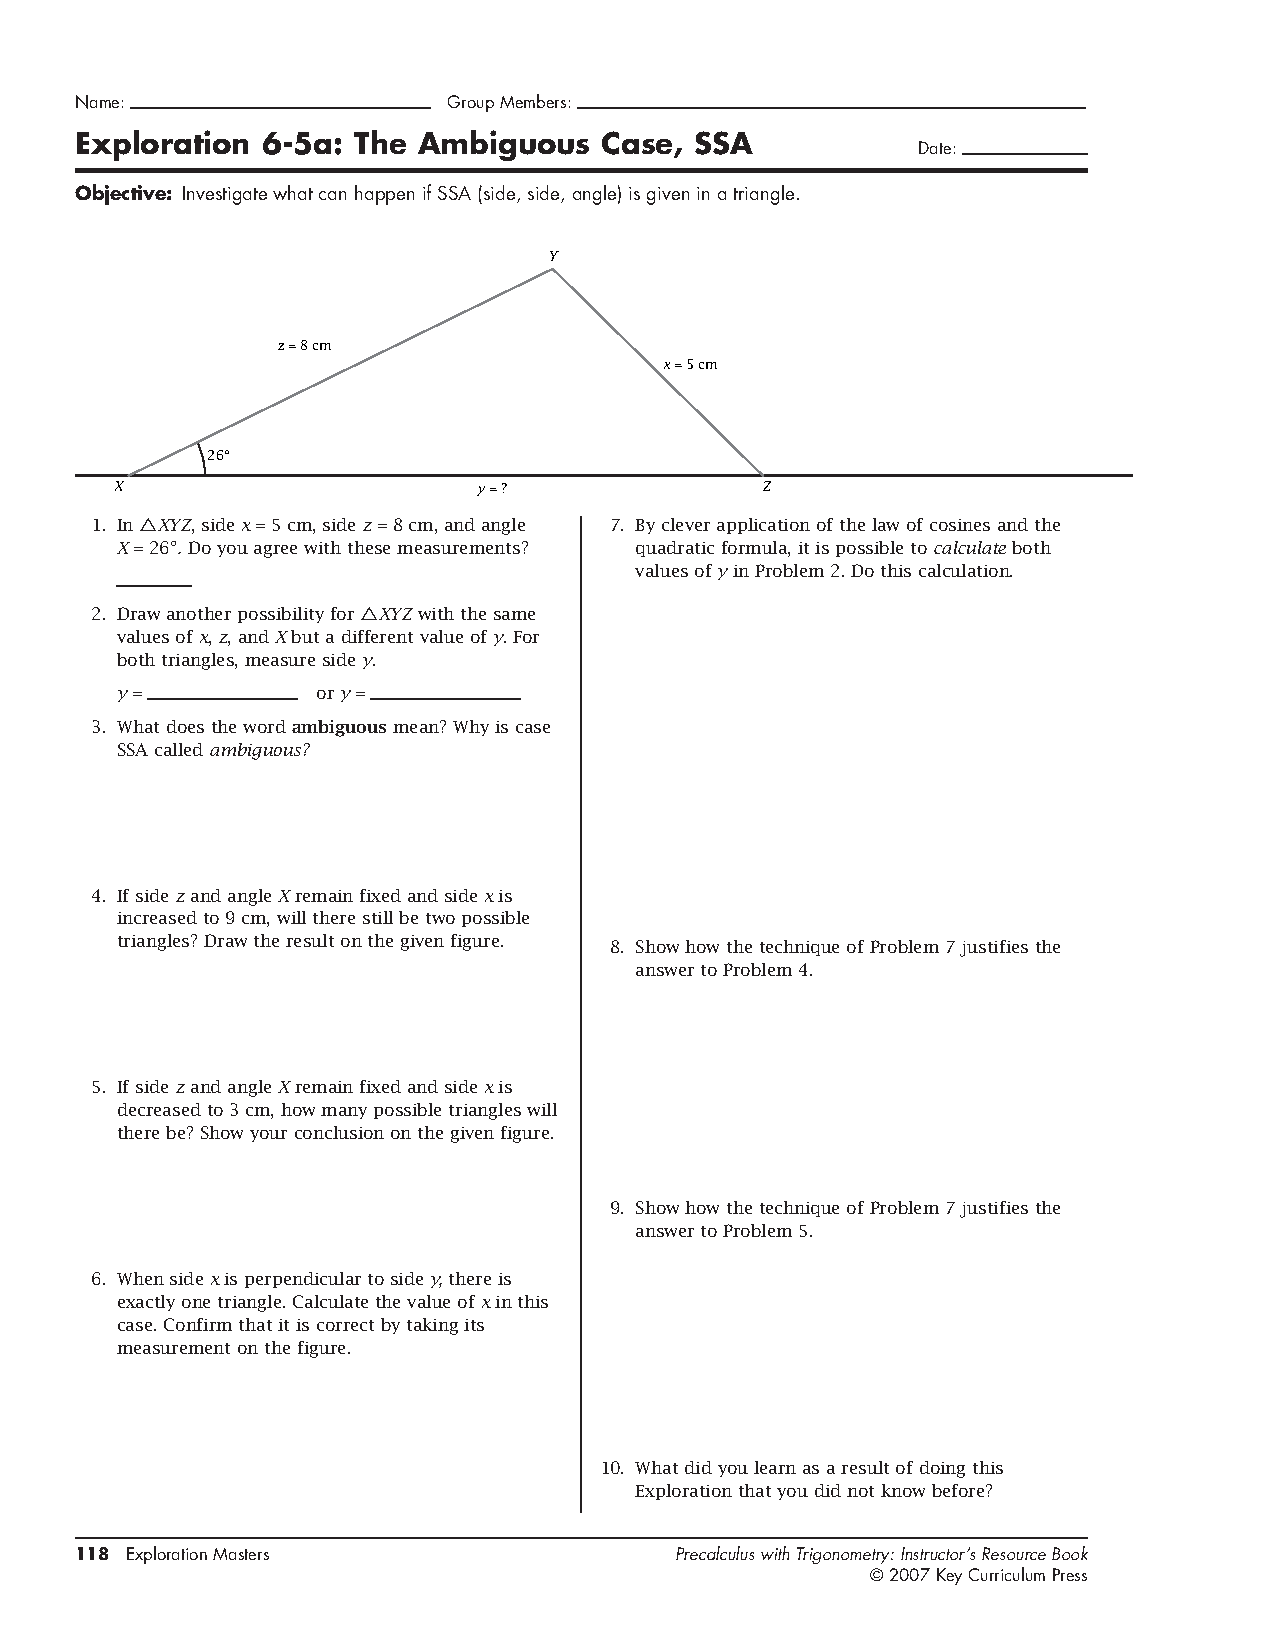
\includegraphics[width=\paperwidth]{ch11/1104p.pdf}}
\newpage
\subsection{SSA}
\subsection{Related Rates}
\subsection{Exercises}
to be done in kuta


%									11 - 5
\newpage
\invisiblesection{2D Vectors}
\subsection{Problems}
\noindent\makebox[\textwidth]{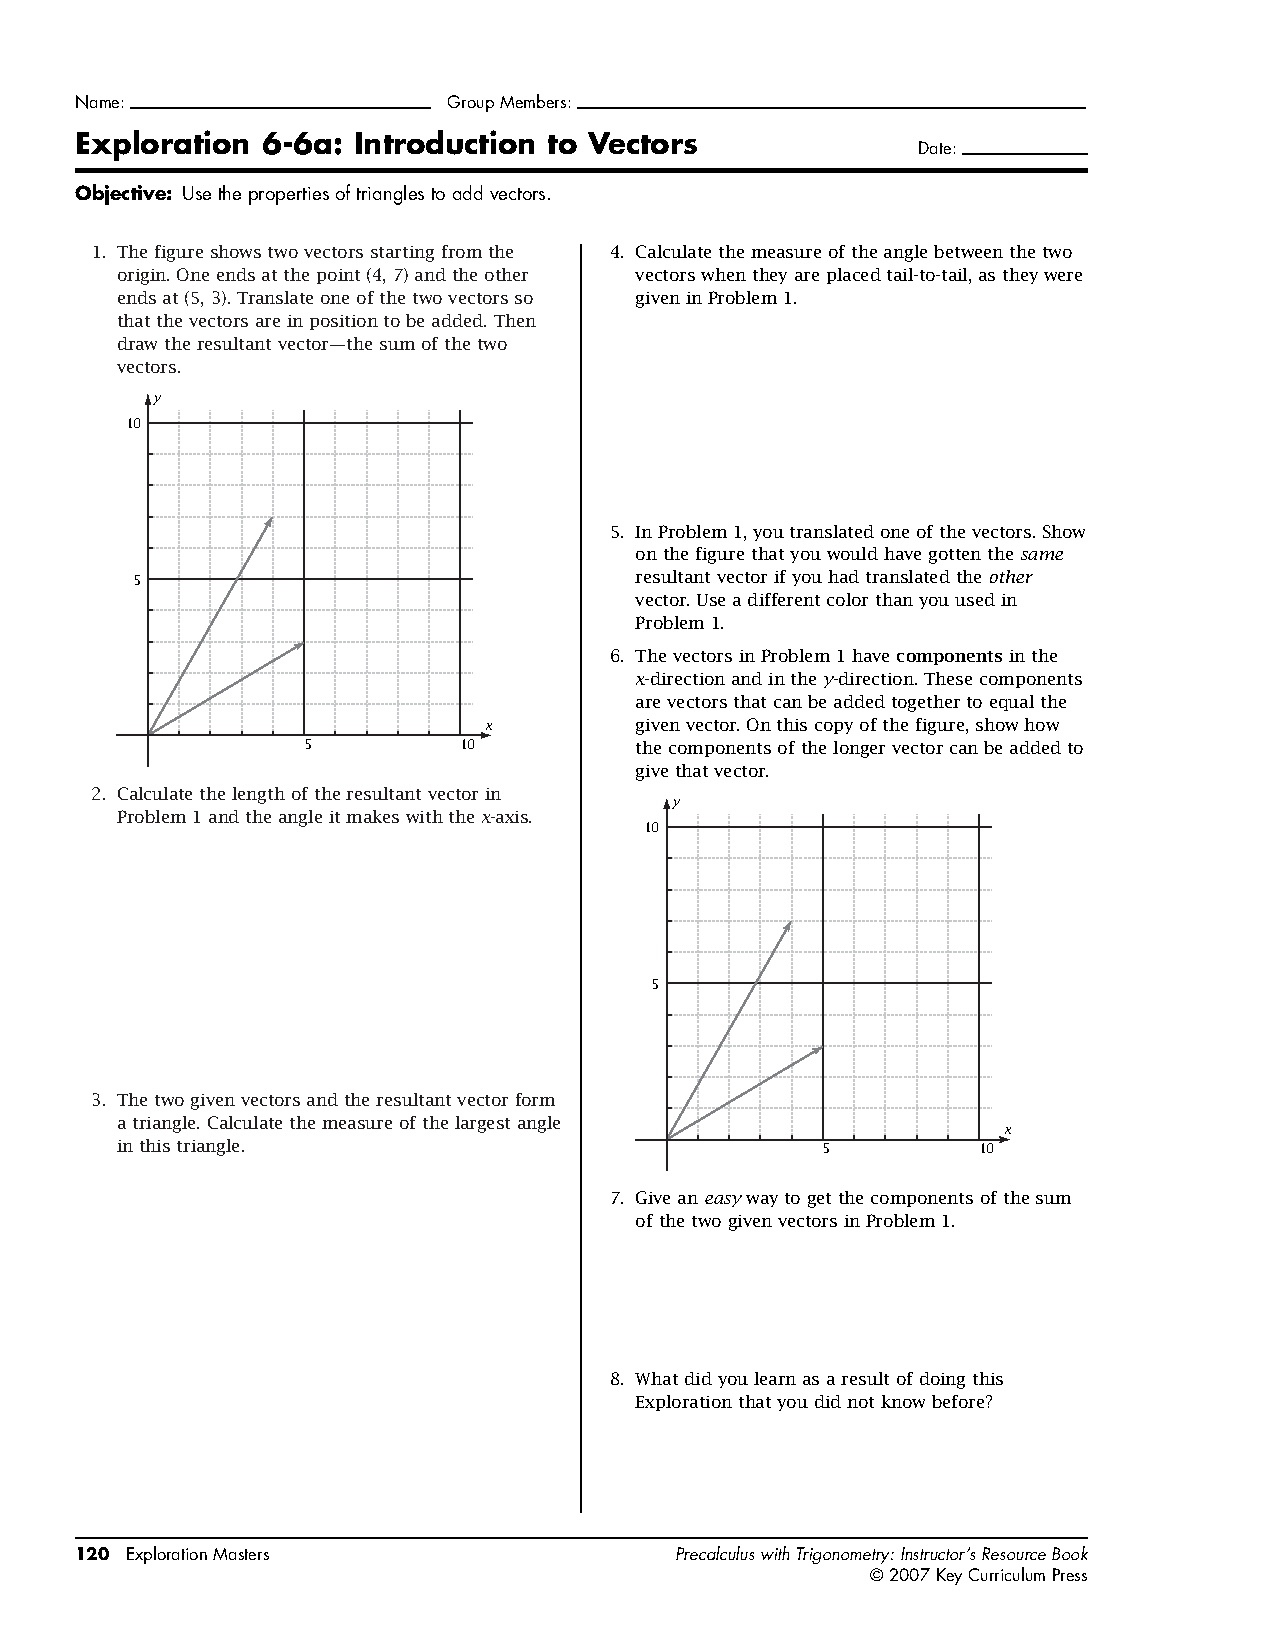
\includegraphics[width=\paperwidth]{ch11/1105p.pdf}}
\newpage
\subsection{Definition and Magnitude}
Vectors have a length, called their magnitude, written with absolute value bars.
\index{Absolute Value!of vectors}
\subsection{Vector Components}
\subsection{Heading and Bearing}
\newpage
\subsection{Exercises}
to be done in kuta

%									11 - 6
\newpage
\section{Review}
\subsection{Chapter Review}
\subsection{Chapter Test}